\begin{figure}[ht!]
	\centering
	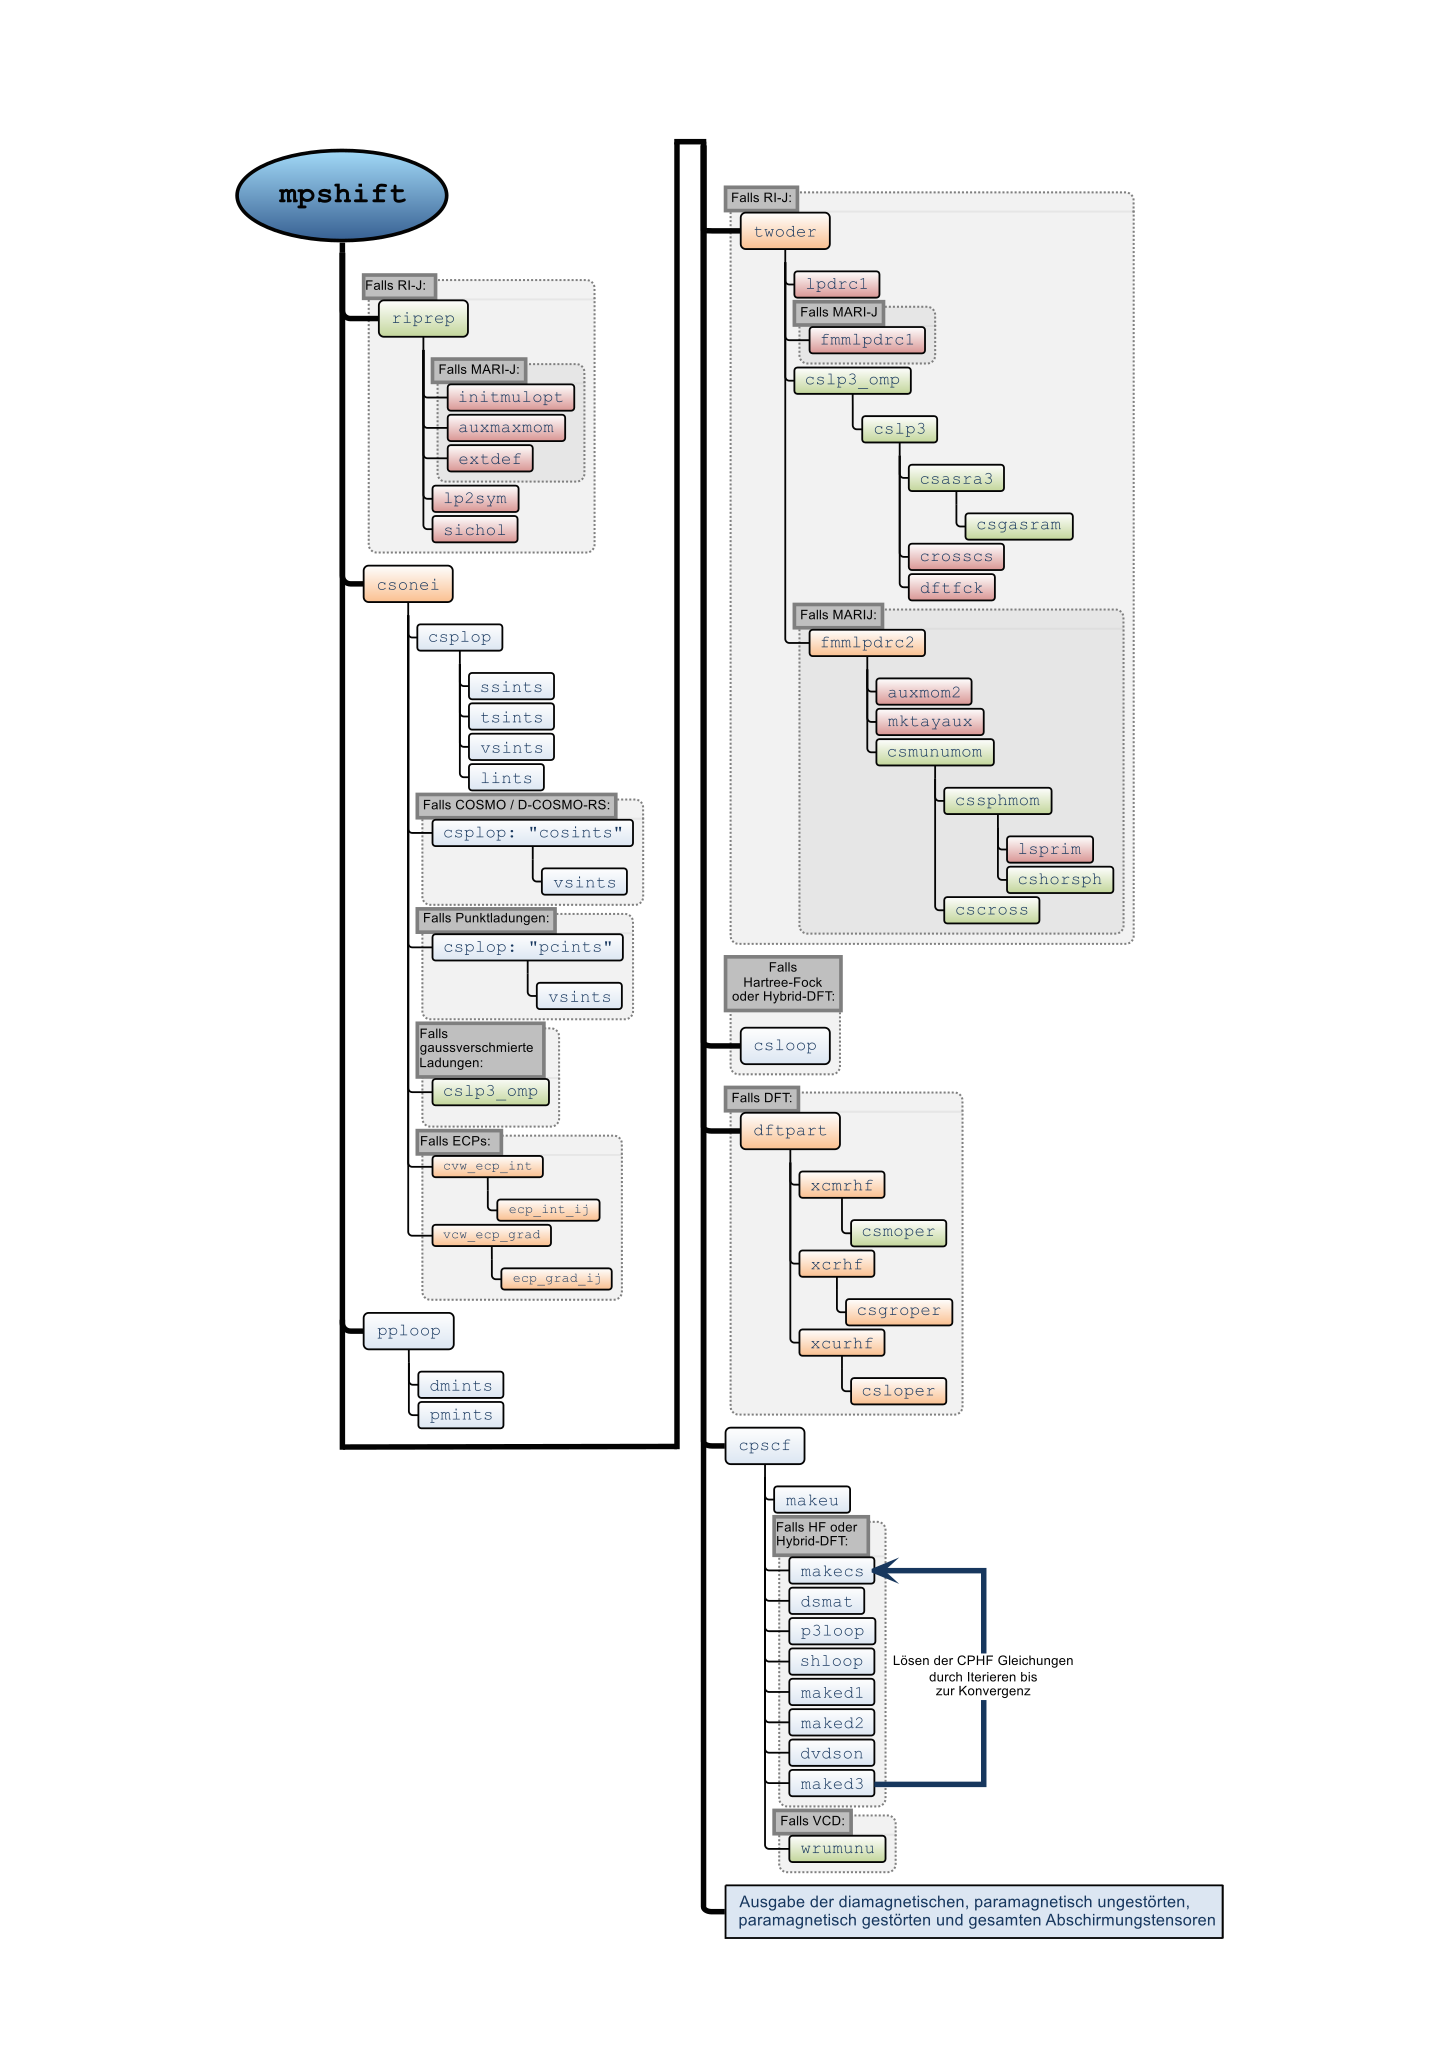
\includegraphics[width=1.0\textwidth]{mpshift_all}
	\captionsetup{figurewithin = chapter}
	\captionsetup{font=small, labelfont=bf}\caption[Neue schematische Programmstruktur des Moduls \texttt{mpshift}]{Schematische Programmstruktur des Moduls \texttt{mpshift} mit den wichtigsten Änderungen und Erweiterungen die im Rahmen der vorliegenden Arbeit durchgeführt wurden. Alte Routinen sind in blau, neue Routinen in grün, modifizierte Routinen in orange und unverändert aus anderen Modulen übertragene Routinen in rot dargestellt.}
\label{abb:neue_programmstruktur}
\end{figure}